% PCT-SOURCE: pdf=086 print=74 kind=figure id=2-5
% Native reconstruction of the two domains meeting the interval [a,b].
\begingroup
\renewcommand{\thefigure}{2-5}
\renewcommand{\figurename}{FIGURE}
\begin{figure}[htbp]
  \centering
  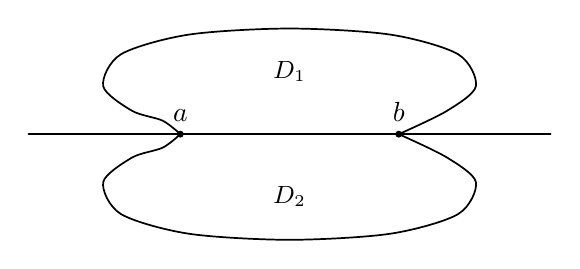
\begin{tikzpicture}[x=1.02cm,y=.78cm,line cap=round,line join=round]
    \draw[line width=.62pt] (-3.25,0) -- (3.25,0);
    \fill (-1.36,0) circle (1.25pt);
    \fill (1.36,0) circle (1.25pt);
    \node[above=1pt] at (-1.36,0) {$a$};
    \node[above=1pt] at (1.36,0) {$b$};
    \draw[line width=.62pt]
      plot[smooth] coordinates {
        (-1.36,0) (-1.58,.22) (-1.96,.38) (-2.32,.78)
        (-2.10,1.30) (-1.26,1.62) (0,1.72) (1.26,1.62)
        (2.10,1.30) (2.32,.78) (1.96,.38) (1.36,0)};
    \draw[line width=.62pt]
      plot[smooth] coordinates {
        (-1.36,0) (-1.58,-.22) (-1.96,-.38) (-2.32,-.78)
        (-2.10,-1.30) (-1.26,-1.62) (0,-1.72) (1.26,-1.62)
        (2.10,-1.30) (2.32,-.78) (1.96,-.38) (1.36,0)};
    \node[font=\small] at (0,1.02) {$D_1$};
    \node[font=\small] at (0,-1.02) {$D_2$};
  \end{tikzpicture}
  \caption{Domains $D_1$ and $D_2$, of definition of $F_1$ and $F_2$,
  respectively.}
  \label{fig:2-5}
  \label{fig:ch2-edge-wedge-domains}
\end{figure}
\endgroup
